\documentclass{article}
\usepackage[utf8]{inputenc}
\usepackage{polski}
\usepackage[polish]{babel}
\usepackage{graphicx}
\usepackage{amsmath}
\usepackage{listings}
\usepackage{hyperref}
\usepackage{float}

\title{POP - Projekt - Sprawozdanie końcowe}
\author{Adam Czupryński \and Szymon Makuch}

\begin{document}
\maketitle

\section{Temat projektu}
Ewolucja różnicowa z modyfikacją wdrażającą nieszablonowy model zastępczy (surrogate model) w celu optymalizacji procesu selekcji osobników z populacji do ewaluacji funkcji celu.

\section{Opis problemu}
Ewolucja różnicowa (DE) jest skutecznym algorytmem optymalizacji globalnej, jednak jej główną wadą jest duża liczba wymaganych ewaluacji funkcji celu. W przypadku gdy obliczenie wartości funkcji celu jest czasochłonne lub kosztowne, może to znacząco ograniczać praktyczne zastosowanie algorytmu. Rozwiązaniem tego problemu może być zastosowanie modelu zastępczego (surrogate model), który aproksymuje wartość funkcji celu na podstawie wcześniej obliczonych punktów.

\section{Implementacja}
\subsection{Struktura projektu}
Projekt został zaimplementowany w języku Python. Główny algorytm ewolucji różnicowej znajduje się w pliku differential\_evolution.py, natomiast jego zmodyfikowana wersja wykorzystująca model zastępczy w surrogate\_de.py. Funkcje testowe z benchmarku CEC oraz pomocnicze funkcje do przeprowadzania eksperymentów znajdują się odpowiednio w plikach functions.py oraz experiments.py. Skrypt plot.py odpowiada za ilustrację średniej liczby ewaluacji i jakości rozwiązań. 

\subsection{Model zastępczy}
W ramach projektu jako model zastępczy stworzyliśmy drzewo regresyjne. Model wykorzystuje algorytm minimalizacji błędu średniokwadratowego (MSE), pozwalając na kontrolę głębokości drzewa i minimalnej liczby próbek w liściach. Implementacja znajduje się w pliku custom\_tree.py.

\section{Eksperymenty i wyniki}

\subsection{Wyznaczanie parametrów algorytmu}
W ramach eksperymentów przeprowadziliśmy analizę wpływu parametrów algorytmu na jego wydajność. W tym celu zmienialiśmy wartości współczynnika mutacji F (0.4-1.0), współczynnika krzyżowania CR (0.3-0.9) oraz rozmiaru populacji (30-100). Wyniki eksperymentów przedstawiono na rysunku:

\begin{figure}[H]
    \centering
    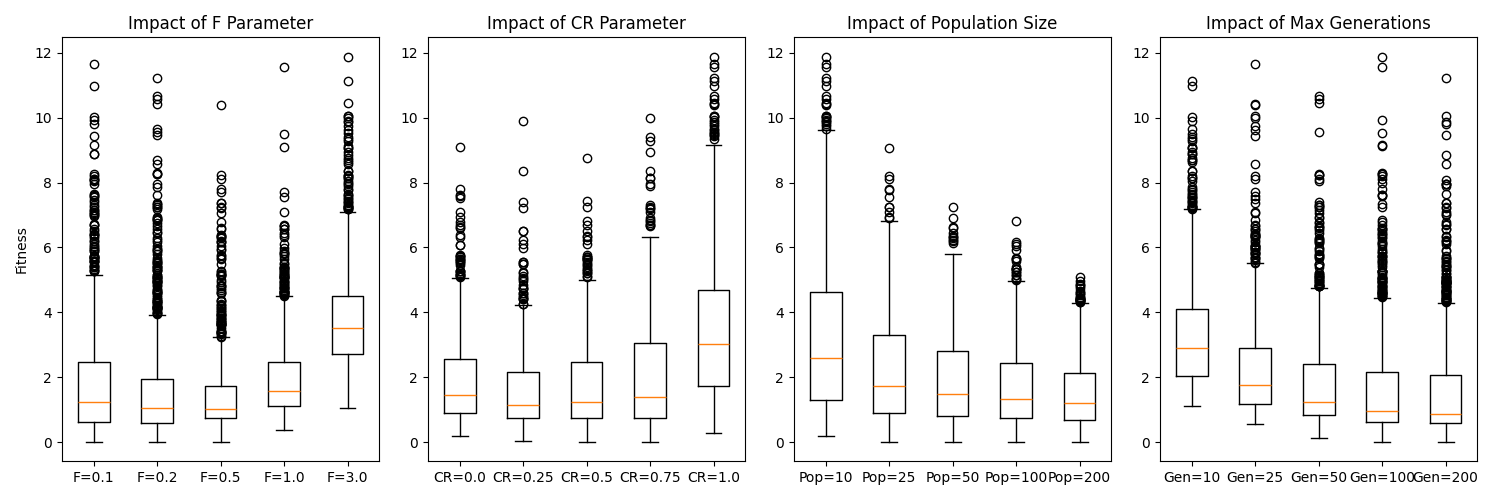
\includegraphics[width=\textwidth]{parameter_tuning_results.png}
    \caption{Wpływ parametrów na jakość algorytmu}
    \label{fig:parameter_results}
\end{figure}

Największe znaczenie na wynik algorytmu ma dobór współczynnika F - dla mniejszych jego wartości wynik był bliższy optimum. Większy rozmiar populacji nieznacznie poprawił wynik działania algorytmu. Wyższe wartości CR prowadzą do lepszej eksploracji przestrzeni rozwiązań.

\subsection{Porównanie liczby ewaluacji funkcji celu}
W celu porównania wydajności standardowego DE z DE przeprowadziliśmy eksperymenty na funkcjach Rosenbrocka i Rastrigina. Wyniki eksperymentów przedstawiono na rysunku:

Dla funkcji Rastrigina:

\begin{figure}[H]
    \centering
    \includegraphics[width=\textwidth]{results_evaluations_rastrigin.png}
    \label{fig:results_evaluations}
\end{figure}

Dla funkcji Rosenbrocka:

\begin{figure}[H]
    \centering
    \includegraphics[width=\textwidth]{results_evaluations_rosenbrock.png}
    \caption{Porównanie liczby ewaluacji funkcji celu}
    \label{fig:results_evaluations}
\end{figure}

Zastosowanie modelu zastępczego pozwoliło na znaczącą redukcję liczby ewaluacji funkcji celu. 

\subsection{Porównanie wydajności}

Do testowania algorytmów wykorzystaliśmy funkcje testowe z benchmarku CEC: Shifted Sphere, Shifted Schwefel, Shifted Rotated Elliptic oraz Shifted Rotated Griewank.

\begin{figure}[H]
    \centering
    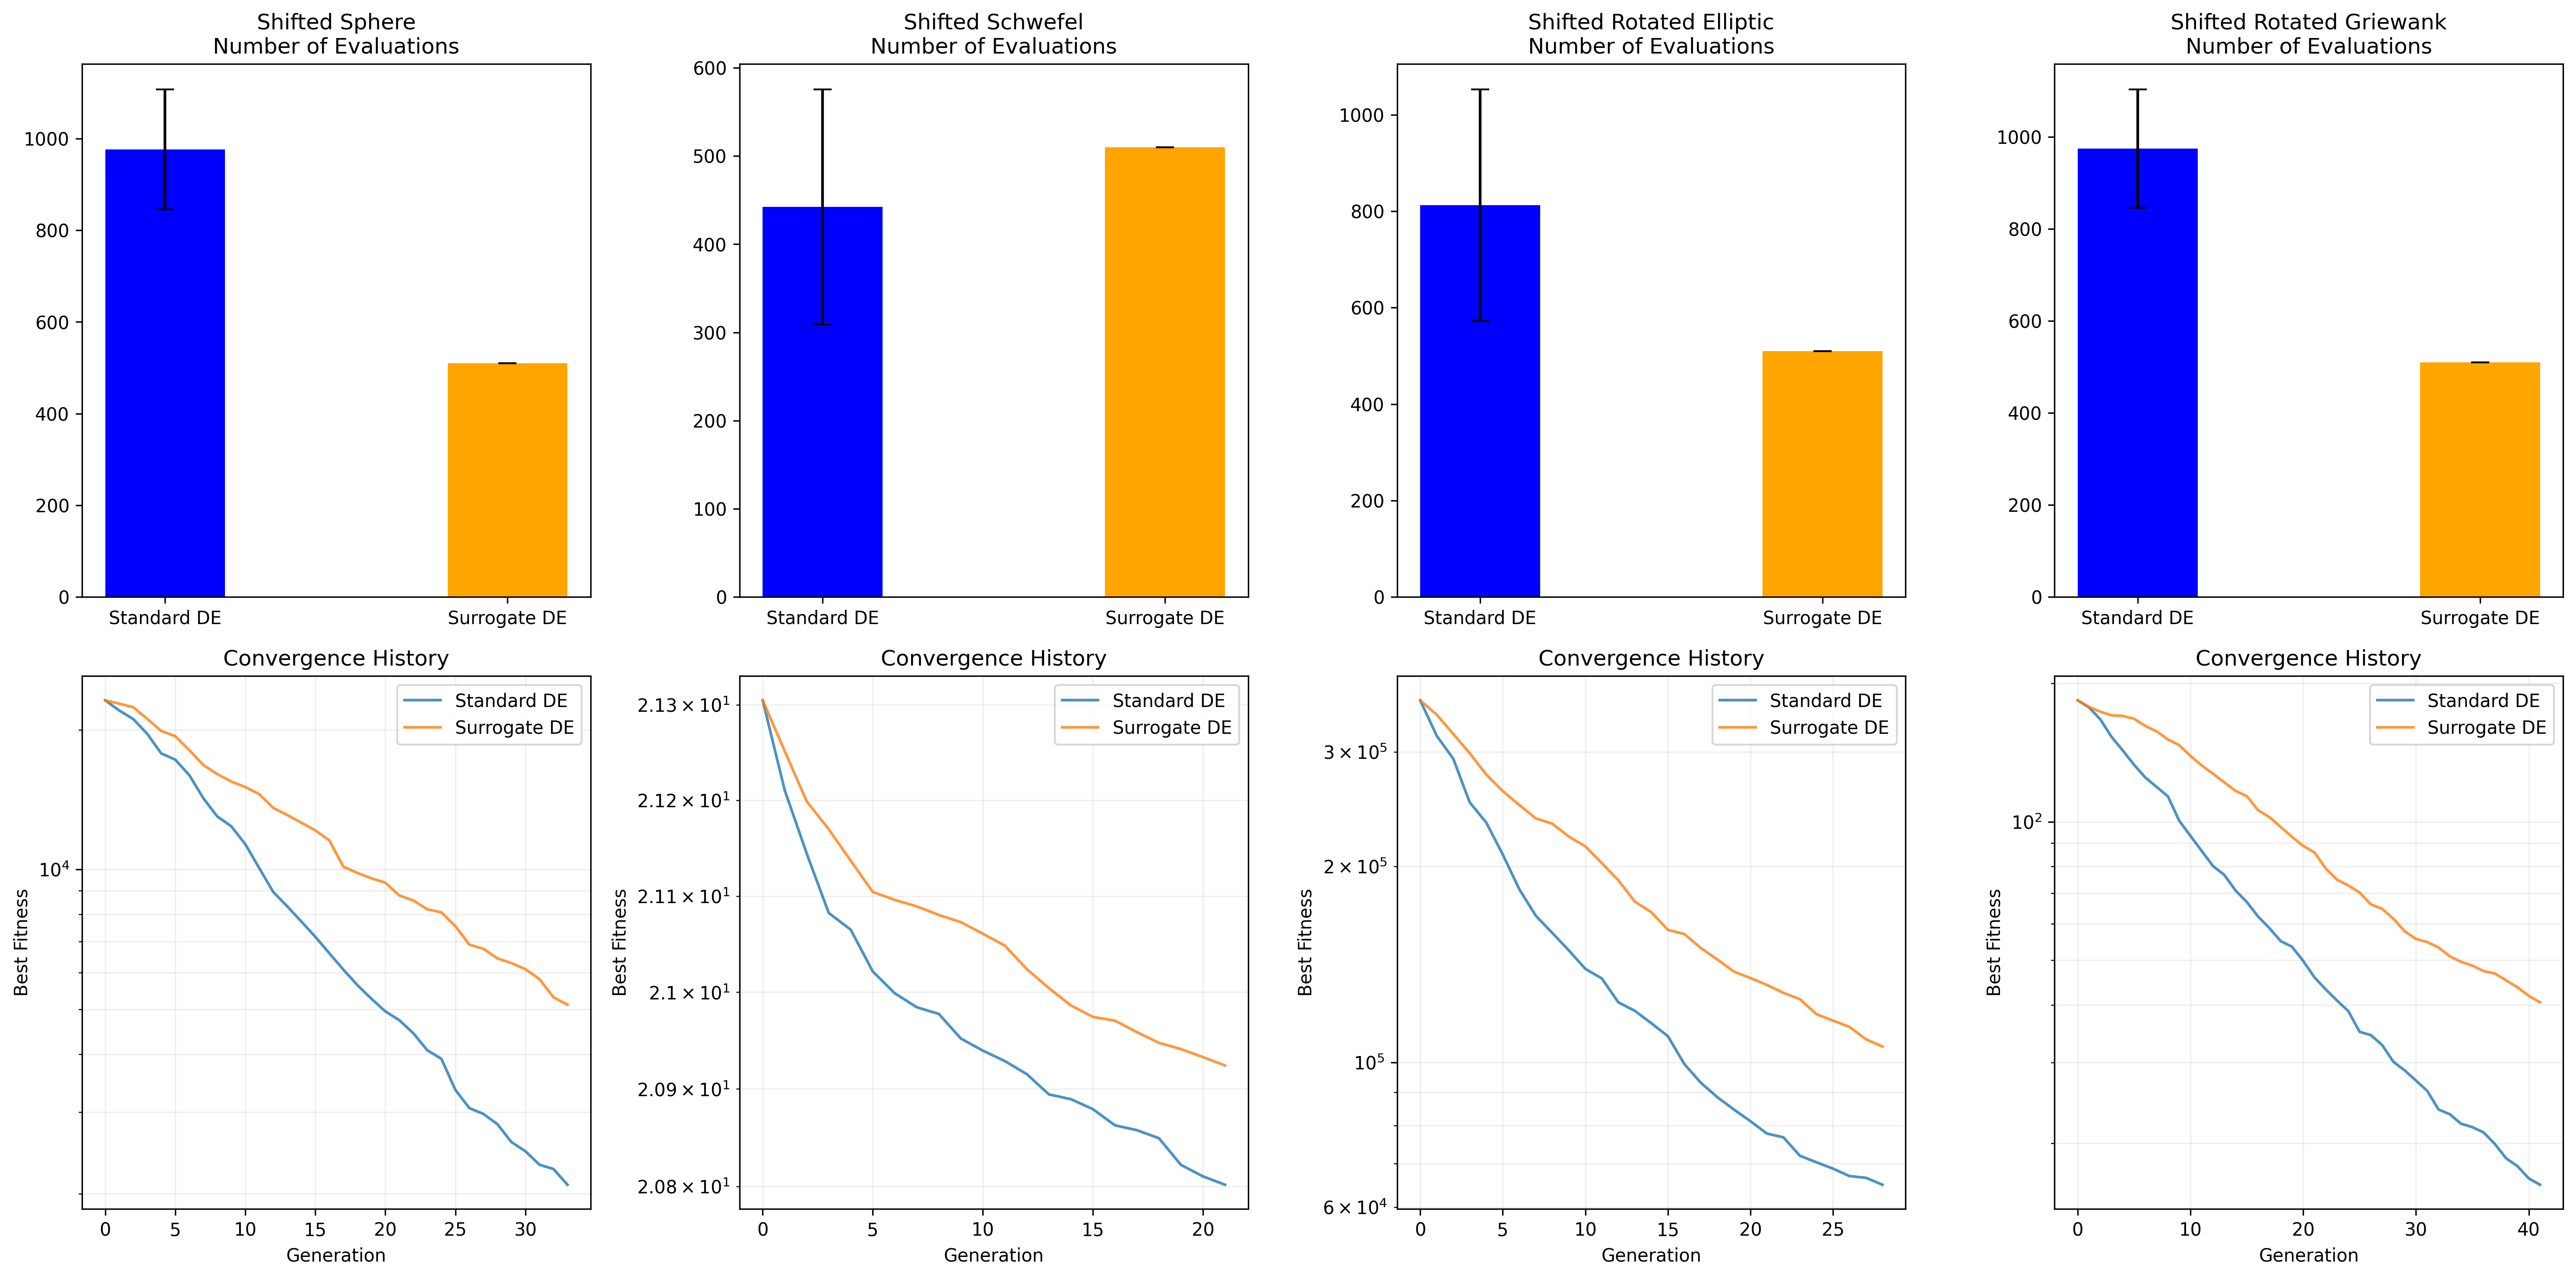
\includegraphics[width=\textwidth]{comprehensive_results.png}
    \caption{Porównanie standardowego DE z DE wykorzystującym model zastępczy}
    \label{fig:comprehensive_results}
\end{figure}

Dla każdej testowanej funkcji, zgodnie z oczekiwaniami, użycie modelu zastępczego dawało gorsze wyniki.

\section{Wnioski}
Przeprowadzone eksperymenty potwierdziły skuteczność zastosowania modelu zastępczego w redukcji liczby ewaluacji funkcji celu, kosztem dokładności zwracanego wyniku.

\end{document}